%==============================================================================
\section{DeltaSort Algorithm}
\label{sec:algorithm}
%==============================================================================

\subsection{Overview}

DeltaSort is a stable\footnote{Strictly speaking, the stability also depends upon the sorting routine used internally to sort updated values. As long as the sorting routine used internally is stable, DeltaSort remains stable as a whole.} update-aware sorting algorithm. It operates in two phases (see~\algoref{alg:deltasort} for pseudocode). The first phase establishes a structure among updated values, and the second phase exploits this structure to efficiently sort the array.

\paragraph{Phase 1: Establish structure} DeltaSort begins by extracting the values at the updated indices, sorting them, and writing them back into the array in increasing index order. This step enforces order among updated positions: if $i < j$ are both updated indices, then $A[i] \le A[j]$ (according to \texttt{cmp}) after Phase~1. The unchanged values are already in order by design. Hence, any remaining order violations must occur only between updated values and their unchanged neighbours.

\paragraph{Phase 2: Fix violations}
With the above structure in place, DeltaSort fixes the array one updated index at a time left to right. When an updated index is first encountered, we first determine its \emph{direction}:

\begin{algorithm}[H]
\caption{DeltaSort}
\label{alg:deltasort}
\begin{algorithmic}[1]
\Require Array $A[0..n-1]$, updated indices $U$, comparator $\texttt{cmp}$
\Ensure $A$ is sorted
\Statex
\State \textbf{Phase 1: Establish segments}
\State $\texttt{updatedIndices} \gets \text{sort}(U)$;
\State $\texttt{updatedValues} \gets \text{sort}([A[u] : u \in \texttt{updatedIndices}], \texttt{cmp})$
\For{$i \gets 0$ \textbf{to} $|\texttt{updatedIndices}| - 1$}
\State $A[\texttt{updatedIndices}[i]] \gets \texttt{updatedValues}[i]$
\EndFor
\State $\texttt{updatedIndices.push}(n)$; \Comment{Sentinel for handling trailing segment with no LEFT's}
\Statex
\State \textbf{Phase 2: Fix segments}
\State $\texttt{pendingRight} \gets []$; $\texttt{leftBound} \gets 0$
\For{$p \gets 0$ \textbf{to} $|\texttt{updatedIndices}| - 1$}
    \State $i \gets \texttt{updatedIndices}[p]$; $\texttt{dir} \gets (i = n)$ ? \textsc{Left} : $\Call{GetDirection}{A, i}$
    \If{$\texttt{dir} = \textsc{Left}$}
        \State $\texttt{rightBound} \gets i - 1$
        \While{$\texttt{pendingRight} \neq \emptyset$}
            \State $j \gets \texttt{pendingRight.pop}()$
            \If{$\texttt{cmp}(A[j], A[j+1]) > 0$}
                \State $\texttt{rightBound} \gets \Call{FixRight}{A, j, \texttt{rightBound}} - 1$
            \EndIf
        \EndWhile
        \If{$i < n$} \Comment{Skip dummy LEFT sentinel}
            \State $\texttt{leftBound} \gets \Call{FixLeft}{A, i, \texttt{leftBound}} + 1$
        \EndIf
    \Else
        \State $\texttt{pendingRight.push}(i)$ \Comment{Defer RIGHT violation}
    \EndIf
\EndFor
\end{algorithmic}
\end{algorithm}

\vspace{0.5em}

\noindent\begin{minipage}{\linewidth}
\begin{algorithmic}[1]
\Function{GetDirection}{$A$, $i$}
    \State \Return $i > 0 \land \texttt{cmp}(A[i-1], A[i]) > 0$ ? \textsc{Left} : \textsc{Right}
\EndFunction
\end{algorithmic}
\end{minipage}

\vspace{0.5em}

\noindent\begin{minipage}{\linewidth}
\begin{algorithmic}[1]
\Function{FixLeft}{$A$, $i$, $\texttt{leftBound}$}
    \State $t \gets \Call{BinarySearchLeft}{A, A[i], \texttt{leftBound}, i-1}$
    \State \Call{Move}{A, i, t}
    \State \Return $t$
\EndFunction
\end{algorithmic}
\end{minipage}

\vspace{0.5em}

\noindent\begin{minipage}{\linewidth}
\begin{algorithmic}[1]
\Function{FixRight}{$A$, $i$, $\texttt{rightBound}$}
    \State $t \gets \Call{BinarySearchRight}{A, A[i], i+1, \texttt{rightBound}}$
    \State \Call{Move}{A, i, t};
    \State \Return $t$
\EndFunction
\end{algorithmic}
\end{minipage}

\begin{definition}[Direction]
\label{def:direction}
During Phase~2, for an index $i \in U$, we define its \emph{direction} based on its local order with its left neighbour:
\begin{enumerate}
  \item \textbf{LEFT ($L$)}: Value is ordered incorrectly to its left neighbour and hence \textbf{must} move left: $i > 0 \text{ and } A[i-1] > A[i]$
  \item \textbf{RIGHT ($R$)}: Value is ordered correctly to its left neighbour or its the first value and hence \textbf{may} move right: $i = 0 \text{ or } A[i-1] \le A[i]$
\end{enumerate}
\end{definition}

A few important things to note about this definition:
\begin{itemize}
  \item Direction captures which side does the target position of an updated index lie relative to its current position. Hence, the notion of direction is not defined (or needed) for unchanged indices ($i \notin U$).
  \item The definition of direction is asymmetric. $L$ requires a strict violation ($A[i-1] > A[i]$), while $R$ includes both violating and non-violating cases, as it may or may not violate order with its right neighbour. This is deliberate because DeltaSort treats all $R$ values identically, so combining these cases simplifies the implementation (see~\algoref{alg:deltasort}).
\end{itemize}

% Example figure showing segmentation with concrete array
\begin{figure}[t]
\centering
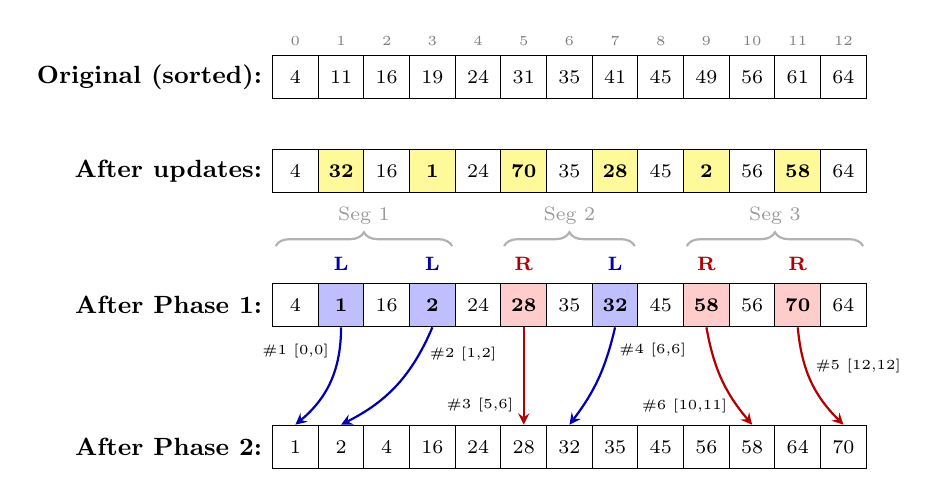
\begin{tikzpicture}[
    cell/.style={draw, minimum width=0.58cm, minimum height=0.55cm, font=\scriptsize},
    cellup/.style={cell, fill=yellow!40, font=\scriptsize\bfseries},
    cellL/.style={cell, fill=blue!25, font=\scriptsize\bfseries},
    cellR/.style={cell, fill=red!20, font=\scriptsize\bfseries},
    larrow/.style={->, >=stealth, thick, blue!70!black},
    rarrow/.style={->, >=stealth, thick, red!70!black},
    segbrace/.style={decorate, decoration={brace, amplitude=5pt}},
]

% === STAGE 1: Original sorted array ===
\node[font=\small\bfseries, anchor=east] at (-0.3, 0) {Original (sorted):};
\foreach \i/\v in {0/4, 1/11, 2/16, 3/19, 4/24, 5/31, 6/35, 7/41, 8/45, 9/49, 10/56, 11/61, 12/64} {
    \node[cell] (o\i) at (\i*0.58, 0) {\v};
}
% Index labels
\foreach \i in {0,...,12} {
    \node[font=\tiny, gray] at (\i*0.58, 0.45) {\i};
}

% === STAGE 2: After updates applied ===
\node[font=\small\bfseries, anchor=east] at (-0.3, -1.2) {After updates:};
\foreach \i/\v/\up in {0/4/0, 1/32/1, 2/16/0, 3/1/1, 4/24/0, 5/70/1, 6/35/0, 7/28/1, 8/45/0, 9/2/1, 10/56/0, 11/58/1, 12/64/0} {
    \ifnum\up=1
        \node[cellup] (u\i) at (\i*0.58, -1.2) {\v};
    \else
        \node[cell] (u\i) at (\i*0.58, -1.2) {\v};
    \fi
}

% === STAGE 3: After Phase 1 (sorted updates, L/R classified) ===
\node[font=\small\bfseries, anchor=east] at (-0.3, -2.9) {After Phase 1:};

% Segment braces (between Stage 2 and L/R labels)
\draw[segbrace, thick, gray!60] (0*0.58-0.25, -2.15) -- (3*0.58+0.25, -2.15) 
    node[midway, above=4pt, font=\scriptsize, gray!80] {Seg 1};
\draw[segbrace, thick, gray!60] (5*0.58-0.25, -2.15) -- (7*0.58+0.25, -2.15) 
    node[midway, above=4pt, font=\scriptsize, gray!80] {Seg 2};
\draw[segbrace, thick, gray!60] (9*0.58-0.25, -2.15) -- (12*0.58+0.25, -2.15) 
    node[midway, above=4pt, font=\scriptsize, gray!80] {Seg 3};

% L/R labels (just above Phase 1 array)
\node[font=\scriptsize, blue!70!black] at (1*0.58, -2.38) {\textbf{L}};
\node[font=\scriptsize, blue!70!black] at (3*0.58, -2.38) {\textbf{L}};
\node[font=\scriptsize, red!70!black] at (5*0.58, -2.38) {\textbf{R}};
\node[font=\scriptsize, blue!70!black] at (7*0.58, -2.38) {\textbf{L}};
\node[font=\scriptsize, red!70!black] at (9*0.58, -2.38) {\textbf{R}};
\node[font=\scriptsize, red!70!black] at (11*0.58, -2.38) {\textbf{R}};

% Phase 1 array: 4, 1, 16, 2, 24, 28, 35, 32, 45, 58, 56, 70, 64
% Only color violation cells (L=blue, R=red), others plain
\node[cell] (p0) at (0*0.58, -2.9) {4};
\node[cellL] (p1) at (1*0.58, -2.9) {1};
\node[cell] (p2) at (2*0.58, -2.9) {16};
\node[cellL] (p3) at (3*0.58, -2.9) {2};
\node[cell] (p4) at (4*0.58, -2.9) {24};
\node[cellR] (p5) at (5*0.58, -2.9) {28};
\node[cell] (p6) at (6*0.58, -2.9) {35};
\node[cellL] (p7) at (7*0.58, -2.9) {32};
\node[cell] (p8) at (8*0.58, -2.9) {45};
\node[cellR] (p9) at (9*0.58, -2.9) {58};
\node[cell] (p10) at (10*0.58, -2.9) {56};
\node[cellR] (p11) at (11*0.58, -2.9) {70};
\node[cell] (p12) at (12*0.58, -2.9) {64};

% === STAGE 4: After Phase 2 (fully sorted) ===
\node[font=\small\bfseries, anchor=east] at (-0.3, -4.7) {After Phase 2:};

% Final sorted: 1, 2, 4, 16, 24, 28, 32, 35, 45, 56, 58, 64, 70
\foreach \i/\v in {0/1, 1/2, 2/4, 3/16, 4/24, 5/28, 6/32, 7/35, 8/45, 9/56, 10/58, 11/64, 12/70} {
    \node[cell] (f\i) at (\i*0.58, -4.7) {\v};
}

% Movement arrows from Phase 1 to Phase 2 (updated values only)
% Labels show: #fix_number (leftBound, rightBound) - placed beside arrows
\draw[larrow, bend left=25] (p1.south) to node[font=\tiny, black, left, pos=0.2] {\#1 [0,0]} (f0.north);
\draw[larrow, bend left=20] (p3.south) to node[font=\tiny, black, right, pos=0.2] {\#2 [1,2]} (f1.north);
\draw[rarrow] (p5.south) to node[font=\tiny, black, left, pos=0.8] {\#3 [5,6]} (f5.north);
\draw[larrow, bend left=12] (p7.south) to node[font=\tiny, black, right, pos=0.2] {\#4 [6,6]} (f6.north);
\draw[rarrow, bend right=15] (p9.south) to node[font=\tiny, black, left, pos=0.8] {\#6 [10,11]} (f10.north);
\draw[rarrow, bend right=20] (p11.south) to node[font=\tiny, black, right, pos=0.35] {\#5 [12,12]} (f12.north);

\end{tikzpicture}
\caption{Segmentation example: An array of size 13 with 6 updates at indices 1, 3, 5, 7, 9, 11. 
In \textbf{Phase~1}, updated values are sorted among themselves and written back to the array. Each value is classified as \textcolor{blue!70!black}{L} or \textcolor{red!70!black}{R}.
In \textbf{Phase~2}, each value is fixed one by one. The label numbers indicate the fixing order, along with the computed left and right bounds for binary search for each updated value.}
\label{fig:delta-sort-example}
\end{figure}

Phase~2 (line ~9--29) processes updated indices from left to right while maintaining a growing sorted prefix. We describe Phase~2 by first establishing a loop invariant and then prove its correctness by showing that the loop invariant holds during initialization and maintenance, and that the array is fully sorted when it terminates.

\subparagraph{State:} We utilise following state information during Phase~2:
\begin{itemize}
  \item \texttt{updatedIndices}: Sorted list of updated indices with a sentinel $n$ appended at the end.
  \item \texttt{leftBound} ($\ell$): The boundary of the sorted prefix, $0$ at the start.
  \item \texttt{pendingRight}: Stack of pending $R$ indices, empty at the start.
\end{itemize}

\subparagraph{Loop invariant:} At the start of each iteration of the loop at line~10, the following conditions hold for index $p$:
\begin{enumerate}
  \item The subarray $A[0..\ell-1]$ is sorted.
  \item There are no $L$ violations in the range $[\ell, {updatedIndices}[p]-1]$.
  \item The stack contains pending $R$ indices within the range $[\ell, \texttt{updatedIndices}[p]-1]$.
  \item If the previous updated index had $L$ direction, then \texttt{pendingRight} is empty.
\end{enumerate}

\subparagraph{Initialization:} The invariant trivially holds at the start of the first iteration ($p = 0$).

\subparagraph{Maintenance:} We will now show that if the invariant holds for $p$, it also holds for $p+1$. Let $i = \texttt{updatedIndices}[p]$ and $\texttt{dir}$ is direction of $i$.

\textbf{Case 1: $\texttt{dir} = L$}
\begin{enumerate}
  \item We first set $\texttt{rightBound} \gets i - 1$. This marks the right boundary beyond which the $R$ values in \texttt{pendingRight} cannot move, because after Phase~1, updated values are ordered and hence cannot cross each other in either directions.
  \item We then flush all pending $R$ indices $j$ in LIFO order. Each $R$ index $j$ is fixed by binary insertion within the range $[j+1, \texttt{rightBound}]$, where $\texttt{rightBound}$ is advanced leftward after each fix to ensure that we search within a minimal range for maximum efficiency. By construction, it is guaranteed that the range $[j+1, \texttt{rightBound}]$ contains no violations and hence binary search can always find the right insertion point. This step preserves condition (3) and (4) of the loop invariant.
  \item After all $R$s are fixed, we fix the current $L$ index $i$ by binary insertion within $[\ell, i-1]$. This range also contains no violations because all $R$ violations are already fixed in the step above and by invariant condition (3), this range contained no $L$ violations to begin with. Finally, we set $\ell \gets$ (insertion point of $i$) $+ 1$. This is not necessary for correctness, but for performance. This preserves the condition (1) and (2) of the loop invariant.
\end{enumerate}

\textbf{Case 2: $\texttt{dir} = R$}
\begin{enumerate}
  \item If \texttt{pendingRight} is empty, this is the first $R$ in a new segment, so we set $\ell \gets i$. This preserves condition (1) and (2) of the loop invariant.
  \item We then push $i$ onto \texttt{pendingRight} for deferred fixing. This preserves condition (3) and (4) of the loop invariant.
\end{enumerate}

\subparagraph{Termination:} The loop processes all values of \texttt{updatedIndices}, including the sentinel index $n$, which is treated as a $L$. Substituting $p = n$ in the invariant conditions, we have:
\begin{itemize}
  \item Condition (1) implies that $A[0..\ell-1]$ is sorted and contains its final values.
  \item Condition (2) implies there are no $L$ violations in the range $[\ell, n-1]$.
  \item Condition (3) and (4) together imply that there are no $R$ violations in the range $[\ell, n-1]$.
  \item Hence we can conclude that the array $A[0..n-1]$ is fully sorted.
\end{itemize}

Figure~\ref{fig:delta-sort-example} illustrates this sequence of operations for a sample array.

Its important to note that even though we are doing repeated binary insertions for fixing violations, the overall data movement is reduced as compared to naive independent binary insertions because the binary search range is smaller. To formalise this we need to understand the structure that emerges from Phase~1. If we picture the updated indices arranged in a sequence of $L$ and $R$ labels, based on their direction when first encountered during Phase~2, we can partition them into \emph{segments}.

\begin{definition}[Segment]
\label{def:segment}
A \emph{segment} is a subarray of $A$ spanning indices $[i, j]$, where $0 \le i \le j < n$, such that:
\begin{enumerate}
  \item Either $i = 0$, or $i \in U$ and has direction label $R$.
  \item Either $j = n - 1$, or $j \in U$ and has direction label $L$.
  \item There exist no updated indices $p, q \in U$ with $i < p < q < j$ such that $p$ is $L$ and $q$ is $R$.
  \item There exist no updated indices $p < i$ and $q > j$ such that $(p, q)$ is also a segment.
\end{enumerate}
\end{definition}

% Figure: Segment structure diagram
\begin{figure}[H]
\centering
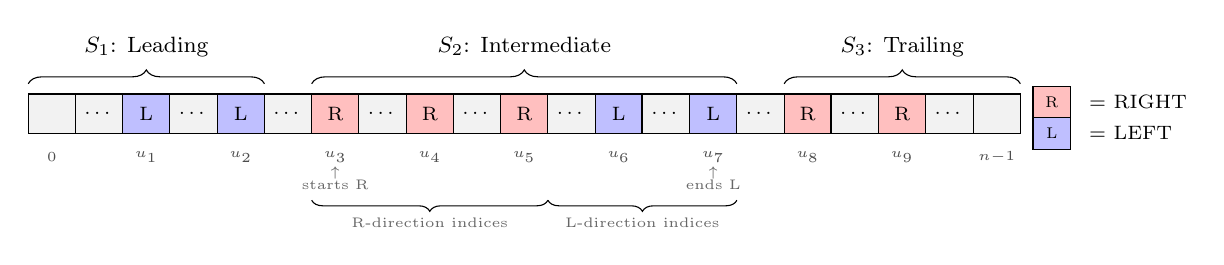
\begin{tikzpicture}[
    cell/.style={minimum width=0.6cm, minimum height=0.5cm, draw, font=\scriptsize},
    dotcell/.style={minimum width=0.5cm, minimum height=0.5cm, font=\scriptsize},
    indexcell/.style={minimum width=0.6cm, font=\tiny, text=black!70},
    right/.style={cell, fill=red!25},
    left/.style={cell, fill=blue!25},
    clean/.style={cell, fill=gray!10, font=\scriptsize},
    segbrace/.style={decorate, decoration={brace, amplitude=5pt}},
    segbracem/.style={decorate, decoration={brace, amplitude=4pt, mirror}},
    seglabel/.style={font=\footnotesize},
    condlabel/.style={font=\tiny, text=black!60},
    faded/.style={opacity=0.4}
]

% Array indices (shown below)
\def\yidx{-0.55}
\def\yarr{0}

% === ARRAY START ===
\node[clean] at (-0.9, \yarr) {};
\node[indexcell] at (-0.9, \yidx) {$0$};
\node[clean] at (-0.3, \yarr) {\dots};

% === LEADING SEGMENT (L's only, bounded by array start) ===
\node[left] (l0) at (0.3, \yarr) {L};
\node[indexcell] at (0.3, \yidx) {$u_1$};
\node[clean] at (0.9, \yarr) {\dots};
\node[left] (l1) at (1.5, \yarr) {L};
\node[indexcell] at (1.5, \yidx) {$u_2$};

% Inter-segment clean region
\node[clean] at (2.1, \yarr) {\dots};

% === MIDDLE SEGMENT (R's then L's) ===
\node[right] (r1) at (2.7, \yarr) {R};
\node[indexcell] at (2.7, \yidx) {$u_3$};
\node[clean] at (3.3, \yarr) {\dots};
\node[right] (r2) at (3.9, \yarr) {R};
\node[indexcell] at (3.9, \yidx) {$u_4$};
\node[clean] at (4.5, \yarr) {\dots};
\node[right] (r3) at (5.1, \yarr) {R};
\node[indexcell] at (5.1, \yidx) {$u_5$};
\node[clean] at (5.7, \yarr) {\dots};
\node[left] (l2) at (6.3, \yarr) {L};
\node[indexcell] at (6.3, \yidx) {$u_6$};
\node[clean] at (6.9, \yarr) {\dots};
\node[left] (l3) at (7.5, \yarr) {L};
\node[indexcell] at (7.5, \yidx) {$u_7$};

% Inter-segment clean region
\node[clean] at (8.1, \yarr) {\dots};

% === TRAILING SEGMENT (R's only, bounded by array end) ===
\node[right] (r4) at (8.7, \yarr) {R};
\node[indexcell] at (8.7, \yidx) {$u_8$};
\node[clean] at (9.3, \yarr) {\dots};
\node[right] (r5) at (9.9, \yarr) {R};
\node[indexcell] at (9.9, \yidx) {$u_9$};

% === ARRAY END ===
\node[clean] at (10.5, \yarr) {\dots};
\node[clean] at (11.1, \yarr) {};
\node[indexcell] at (11.1, \yidx) {$n{-}1$};

% === SEGMENT BRACES (top) ===
% Leading segment
\draw[segbrace] (-1.2, 0.38) -- (1.8, 0.38);
\node[seglabel] at (0.3, 0.85) {$S_1$: Leading};

% Middle segment
\draw[segbrace] (2.4, 0.38) -- (7.8, 0.38);
\node[seglabel] at (5.1, 0.85) {$S_2$: Intermediate};

% Trailing segment
\draw[segbrace] (8.4, 0.38) -- (11.4, 0.38);
\node[seglabel] at (9.9, 0.85) {$S_3$: Trailing};

% === SUB-BRACES for middle segment (bottom) ===
\draw[segbracem] (2.4, -1.1) -- (5.4, -1.1);
\node[condlabel, anchor=north] at (3.9, -1.2) {R-direction indices};
\draw[segbracem] (5.4, -1.1) -- (7.8, -1.1);
\node[condlabel, anchor=north] at (6.6, -1.2) {L-direction indices};

% === ANNOTATIONS for boundary conditions ===
% Condition markers (centered on cells)
\node[condlabel] at (2.7, -0.75) {$\uparrow$};
\node[condlabel] at (2.7, -0.9) {starts R};

\node[condlabel] at (7.5, -0.75) {$\uparrow$};
\node[condlabel] at (7.5, -0.9) {ends L};

% === LEGEND ===
\node[right, scale=0.8] at (11.8, 0.15) {R};
\node[font=\scriptsize, anchor=west] at (12.15, 0.15) {= RIGHT};
\node[left, scale=0.8] at (11.8, -0.25) {L};
\node[font=\scriptsize, anchor=west] at (12.15, -0.25) {= LEFT};

\end{tikzpicture}
\caption{A segment $(i,j)$ starts at either index $0$ or an R-direction updated index, and ends at either index $n{-}1$ or an L-direction updated index, with all R's preceding all L's within. In this example, the leading segment $S_1$ contains only L's (starting from index $0$), the intermediate segment $S_2$ contains R's followed by L's, and the trailing segment $S_3$ contains only R's (ending at index $n{-}1$). Leading and trailing segments may or may not be present depending on the directions of updated indices.}
\label{fig:segment-structure}
\end{figure}

More intuitively, a segment is a maximal contiguous region of the array in which all $R$-direction updates precede all $L$-direction updates. The first two conditions define valid segment boundaries, the third enforces the $R^\ast L^\ast$ structure within a segment, and the final condition ensures that segments are maximal and non-overlapping. \figref{fig:segment-structure} illustrates this structure.

\subparagraph{Key Insight: Segments can be fixed \emph{locally} and \emph{independently}:}
\label{sec:insight}

Unlike naive BIS, where each insertion can be at any point in the array, in DeltaSort, \emph{an updated value in a segment cannot cross its segment boundary}. We formally prove this property next.

\begin{lemma}[Movement Confinement]
\label{lem:confinement}
During Phase~2, all value movement is confined within segment boundaries.
\end{lemma}

\begin{proof}
Let $S$ be a segment with $R$-indices $R_0,\ldots,R_{r-1}$ followed by $L$-indices $L_0,\ldots,L_{l-1}$, where $r+l \ge 1$. After Phase~1, updated values are ordered: $A[R_0] \le \cdots \le A[R_{r-1}] \le A[L_0] \le \cdots \le A[L_{l-1}]$. An $R$-value couldn't have crossed $L_0$ (if it exists), and an $L$-value couldn't have crossed $R_{r-1}$ (if it exists), since the above ordering must be preserved. Therefore, no value exits its segment.
\end{proof}

\begin{remark}
  Note that Lemma~\ref{lem:confinement} also implies \emph{segment independence}. Because no value exits its segment, segment lengths don't change. As a result, movement in a segment does not interfere with movement in another segment, which implies segments can be fixed independently in any order. This opens up opportunities for \textbf{parallelization} that can improve performance even further on multi-core systems and distributed environments. To avoid expanding scope, we leave this investigation for future work.
\end{remark}

\subsection{Complexity Analysis}
\label{sec:complexity}

We analyse the expected total data movement incurred during Phase~2 of DeltaSort under a random bounded-range update model. In this model, updated values are drawn uniformly at random from a \emph{fixed} value range. Choosing values at random avoids introducing any special structure that could bias the analysis.

\begin{remark}[Choice of Update Model]
\label{rem:update-model}
Several update models could be considered. For example, a \emph{bounded rank displacement} model constrains updates such that for every updated value $|Rank_{\text{new}} - Rank_{\text{old}}| \le b$ for some bound $b$, while a \emph{clustered update} model restricts updated indices to a region with $u_{\max} - u_{\min} \le c$. Different models interact with DeltaSort’s structure in different ways: bounded displacement directly limits movement and is therefore favorable, whereas clustered updates may either help or hinder performance depending on the induced directional pattern. In this work, we adopt a \emph{random update model} as a neutral baseline. Specifically, updated indices are chosen uniformly at random from $\{0, \ldots, n-1\}$, and updated values are drawn independently from a fixed range of permissible values. This model introduces no additional structure that the algorithm can exploit, nor does it adversarially bias updates towards worst-case configurations (see~\figref{fig:worst-case} for an example of a worst case). Analysing DeltaSort under more structured update models is left to future work.
\end{remark}

\begin{lemma}[Expected Movement]
\label{lem:movement-bound}
Under the random bounded-range update model, for an array of size $n$ with $k$ updated indices, the expected total data movement incurred during DeltaSort's Phase~2 is $O(n \sqrt{k})$.
\end{lemma}

\begin{proof}
After Phase~1, we have two sorted sequences of $k$ values each:
\begin{itemize}
  \item \textbf{Indices:} The $k$ updated positions $i_0 < i_1 < \cdots < i_{k-1}$, sorted.
  \item \textbf{Values:} The $k$ updated values $v_0 \le v_1 \le \cdots \le v_{k-1}$, sorted.
\end{itemize}
After Phase~1, we have two sorted sequences of $k$ values each which forms an \emph{order statistic} of $k$ uniform samples. Using a result from order statistic theory~\cite{feller1968}, we can prove that the number of segments formed are $O(\sqrt{k})$ (see~\lemref{lem:expected-segments} for full proof).

With $O(\sqrt{k})$ segments partitioning the array of size $n$, the expected width of each segment is $O(n / \sqrt{k})$. By \lemref{lem:confinement}, movement is confined within segments. Since each of the $k$ updated values moves at most the width of its containing segment, the expected total movement is:
\[
\mathbb{E}[\text{total movement}] \le k \cdot O\!\left(\frac{n}{\sqrt{k}}\right) = O(n\sqrt{k}) \qedhere
\]
\end{proof}

\begin{remark}[Worst Case Movement]
While the expected movement is $O(n\sqrt{k})$, the worst-case movement can be as high as $O(kn)$. This occurs when updated values form a single segment spanning the entire array. This happens when updates \emph{cluster monotonically} at the start or end of the array (see~\appref{sec:appendix-worst-case} for an illustration). Hence, in a practical setting, a hybrid algorithm will need to fallback to ESM or full re-sort based on the number of segments.
\end{remark}

\begin{lemma}[Comparison Count]
\label{lem:comparison-count}
DeltaSort performs $O(k \log n)$ comparisons.
\end{lemma}

\begin{proof}
Phase~1 sorts the $k$ updated values, requiring $O(k \log k)$ comparisons. In Phase~2, each updated value is fixed using binary search within its containing segment. By \lemref{lem:movement-bound}, the expected number of segments is $O(\sqrt{k})$, so the expected width of a segment is $O(n/\sqrt{k})$. Since searches are confined within segment boundaries, each fix requires $O(\log (n/\sqrt{k}))$ comparisons, for a total of $O(k \log (n/\sqrt{k}))$ comparisons in Phase~2. Summing both gives:
\[
O(k \log k) + O(k \log (n/\sqrt{k})) = O\!\bigl(k(\log k + \log n - \tfrac{1}{2}\log k)\bigr) = O(k \log n) \qedhere
\]
\end{proof}

\begin{theorem}[Time Complexity]
\label{thm:time-complexity}
Under the random bounded-range update model, DeltaSort runs in $O(k \log n + n\sqrt{k})$ expected time.
\end{theorem}

\begin{proof}
By \lemref{lem:movement-bound}, the expected total data movement is $O(n\sqrt{k})$. By \lemref{lem:comparison-count}, the total number of comparisons is $O(k \log n)$. Phase~1 also incurs $O(k \log k)$ movement cost for sorting $k$ values. Combining all we get: $O(k \log n + n\sqrt{k})$.
\end{proof}

\begin{theorem}[Space Complexity]
\label{thm:space}
DeltaSort uses $O(k)$ auxiliary space.
\end{theorem}

\begin{proof}
Phase~1 sorts $k$ values using $O(k)$ space. Phase~2 maintains a pending stack of at most $k$ indices. Therefore, the total auxiliary space is $O(k)$.
\end{proof}